\chapter[Planejamento do Projeto]{Planejamento do Projeto}

O sucesso do projeto é totalmente dependente de uma atividade de planejamento adequada. Nesta atividade, define-se um cronograma de acordo com as características do projeto, como recursos e tempo. É importante respeitar o que foi definido mantendo o fluxo e disciplina nas entregas do projeto.

\section{Cronograma}

A elaboração do cronograma foi realizada utilizando-se as ferramentas Trello e Ganttify. Foram estabelecidos três níveis de atividades: Portfólio, Programa e Time, de acordo com o processo SAFe, tal conjunto de atividades abrange as duas entregas do trabalho. 
A primeira entrega compreende o planejamento, definição de abordagem, processos, ferramentas e técnicas de elicitação de requisitos, referentes ao nível Portfólio.
A segunda entrega do projeto compreende a evolução do processo do cliente, levantamento de requisitos e planejamento e execução de uma sprint, tais atividades são referentes aos níveis de Programa e Time. A figura \ref{cronograma} ilustra o cronograma do projeto.

\begin{figure}[!htbp]
	\centering
	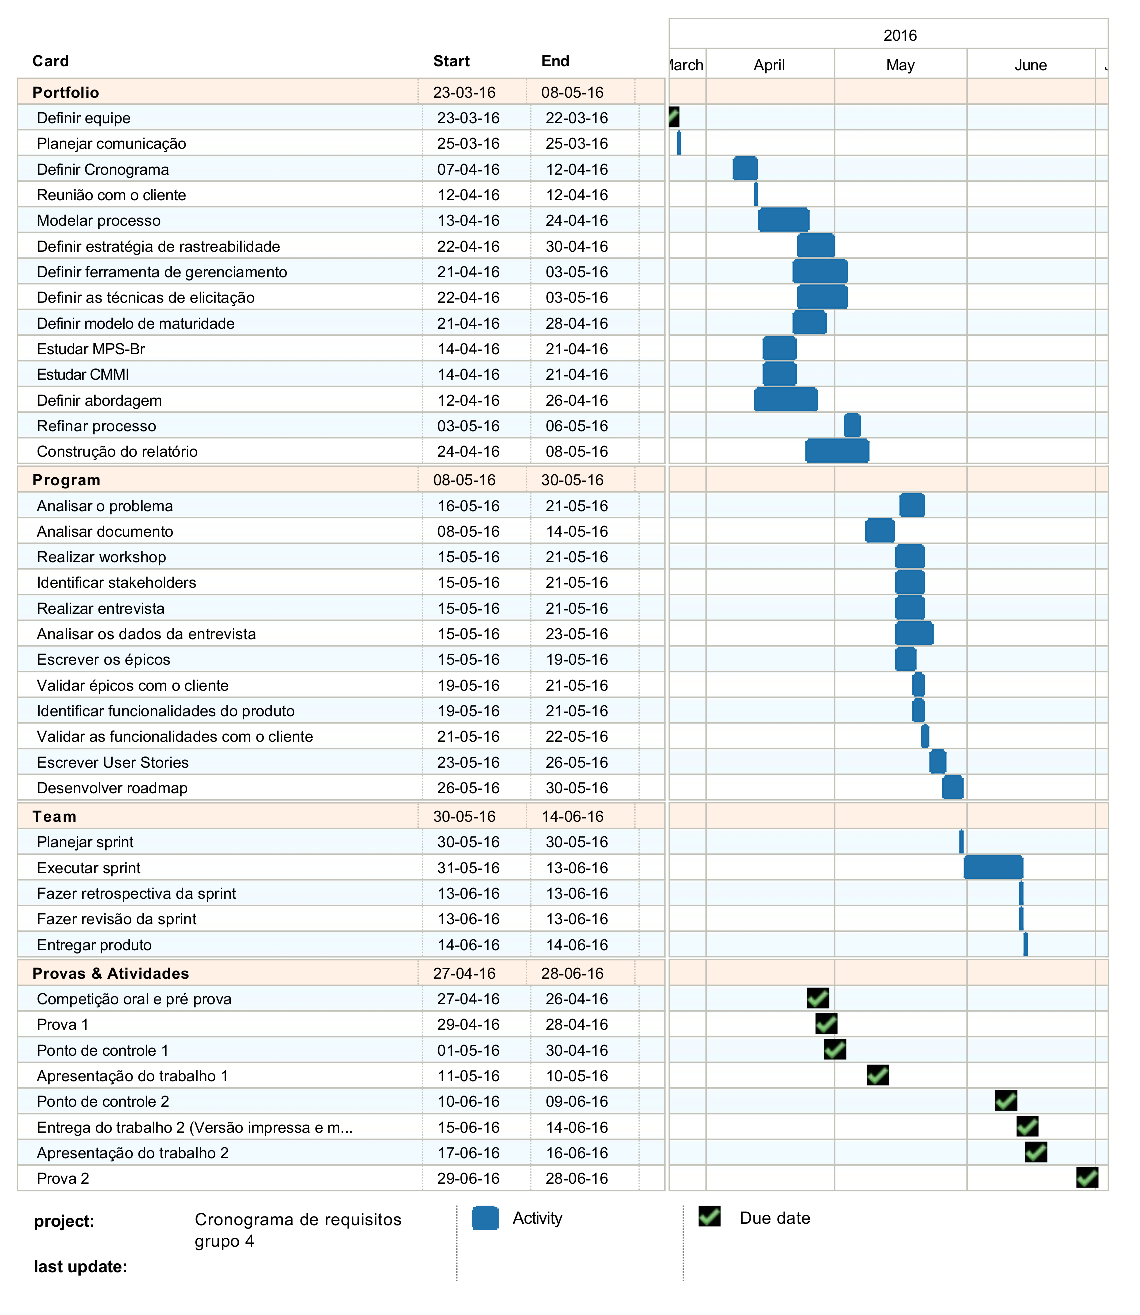
\includegraphics[width=\textwidth]{figuras/cronograma}
	\caption{Planejamento do projeto: cronograma.}
	\label{cronograma}
\end{figure}
